% This is samplepaper.tex, a sample chapter demonstrating the
% LLNCS macro package for Springer Computer Science proceedings;
% Version 2.20 of 2017/10/04
%
\documentclass[runningheads]{llncs}
%

\let\proof\relax
\let\endproof\relax
\let\example\relax
\let\endexample\relax


\usepackage{graphicx}
\usepackage{amsmath, amssymb,amsthm}
\usepackage{tikz}
\usetikzlibrary{arrows.meta,chains,decorations.pathreplacing}


\newtheorem*{theorem*}{Theorem}
%\newtheorem*{definition*}{Definition}
%\newtheorem*{proposition*}{Proposition}
%\newtheorem*{corollary*}{Corollary}
%\newtheorem{observation}{Observation}

%\newtheorem{theorem}{Theorem}
%\newtheorem{lemma}{Lemma}
%\newtheorem{definition}{Definition}
%\newtheorem{corollary}{Corollary}
%\newtheorem{claim}{Claim}
%\newtheorem{proposition}{Proposition}
%\newcommand{\citet}[1]{\cite{#1}}


%\usepackage{thm-restate}

%\declaretheorem[name=Theorem, sibling=theorem]{rThm}
%\declaretheorem[name=Lemma, sibling=lemma]{rLem}
%\declaretheorem[name=Corollary, sibling=corollary]{rCor}
%\declaretheorem[name=Proposition, sibling=theorem]{rPro}
\usepackage{thm-restate}

%\usepackage[sectionbib,numbers]{natbib}

\usepackage{natbib}  % DO NOT CHANGE THIS AND DO NOT ADD ANY OPTIONS TO IT
% Used for displaying a sample figure. If possible, figure files should
% be included in EPS format.
%
% If you use the hyperref package, please uncomment the following line
% to display URLs in blue roman font according to Springer's eBook style:
% \renewcommand\UrlFont{\color{blue}\rmfamily}
%TODO
\newcommand{\todo}[1]{{\color{red}{\bf [TODO]:~{#1}}}}

%THEOREMS
\newtheorem{theorem}{Theorem}
\newtheorem{corollary}{Corollary}
\newtheorem{lemma}{Lemma}
\newtheorem{proposition}{Proposition}
\newtheorem{problem}{Problem}
\newtheorem{definition}{Definition}
\newtheorem{remark}{Remark}
\newtheorem{example}{Example}
\newtheorem{assumption}{Assumption}

%HANS' CONVENIENCES
\newcommand{\define}[1]{\textit{#1}}
\newcommand{\join}{\vee}
\newcommand{\meet}{\wedge}
\newcommand{\bigjoin}{\bigvee}
\newcommand{\bigmeet}{\bigwedge}
\newcommand{\jointimes}{\boxplus}
\newcommand{\meettimes}{\boxplus'}
\newcommand{\bigjoinplus}{\bigjoin}
\newcommand{\bigmeetplus}{\bigmeet}
\newcommand{\joinplus}{\join}
\newcommand{\meetplus}{\meet}
\newcommand{\lattice}[1]{\mathbf{#1}}
\newcommand{\semimod}{\mathcal{S}}
\newcommand{\graph}{\mathcal{G}}
\newcommand{\nodes}{\mathcal{V}}
\newcommand{\agents}{\{1,2,\dots,N\}}
\newcommand{\edges}{\mathcal{E}}
\newcommand{\neighbors}{\mathcal{N}}
\newcommand{\Weights}{\mathcal{A}}
\renewcommand{\leq}{\leqslant}
\renewcommand{\geq}{\geqslant}
\renewcommand{\preceq}{\preccurlyeq}
\renewcommand{\succeq}{\succcurlyeq}
\newcommand{\Rmax}{\mathbb{R}_{\mathrm{max}}}
\newcommand{\Rmin}{\mathbb{R}_{\mathrm{min}}}
\newcommand{\Rext}{\overline{\mathbb{R}}}
\newcommand{\R}{\mathbb{R}}
\newcommand{\N}{\mathbb{N}}
\newcommand{\A}{\mathbf{A}}
\newcommand{\B}{\mathbf{B}}
\newcommand{\x}{\mathbf{x}}
\newcommand{\e}{\mathbf{e}}
\newcommand{\X}{\mathbf{X}}
\newcommand{\W}{\mathbf{W}}
\newcommand{\weights}{\mathcal{W}}
\newcommand{\alternatives}{\mathcal{X}}
\newcommand{\xsol}{\bar{\mathbf{x}}}
\newcommand{\y}{\mathbf{y}}
\newcommand{\Y}{\mathbf{Y}}
\newcommand{\z}{\mathbf{z}}
\newcommand{\Z}{\mathbf{Z}}
\renewcommand{\a}{\mathbf{a}}
\renewcommand{\b}{\mathbf{b}}
\newcommand{\I}{\mathbf{I}}
\DeclareMathOperator{\supp}{supp}
\newcommand{\Par}[2]{\mathcal{P}_{{#1} \to {#2}}}
\newcommand{\Laplacian}{\mathcal{L}}
\newcommand{\F}{\mathcal{F}}
\newcommand{\inv}[1]{{#1}^{\sharp}}
\newcommand{\energy}{Q}
\newcommand{\err}{\mathrm{err}}
\newcommand{\argmin}{\mathrm{argmin}}
\newcommand{\argmax}{\mathrm{argmax}}
\begin{document}
%
\title{Prophet Inequality with Competing Agents}
%
%\titlerunning{Abbreviated paper title}
% If the paper title is too long for the running head, you can set
% an abbreviated paper title here
%
%\author{}
%\institute{}
\author{Tomer Ezra\inst{1} \and
Michal Feldman\inst{1,2} \and
Ron Kupfer\inst{3}}

\authorrunning{Ezra et al.}
% First names are abbreviated in the running head.
% If there are more than two authors, 'et al.' is used.
%
\institute{Tel Aviv University, Israel\\ \and
Microsoft Research\\
\and
The Hebrew University of Jerusalem, Israel\\
\email{tomer.ezra@gmail.com}, 
\email{michal.feldman@cs.tau.ac.il}, 
\email{kupfer.ron@gmail.com}}

\maketitle              % typeset the header of the contribution
%
\begin{abstract}
  In this paper, we explore the connection between secret key agreement and secure omniscience within the setting of the multiterminal source model with a wiretapper who has side information. While the secret key agreement problem considers the generation of a maximum-rate secret key through public discussion, the secure omniscience problem is concerned with communication protocols for omniscience that minimize the rate of information leakage to the wiretapper. The starting point of our work is a lower bound on the minimum leakage rate for omniscience, $\rl$, in terms of the wiretap secret key capacity, $\wskc$. Our interest is in identifying broad classes of sources for which this lower bound is met with equality, in which case we say that there is a duality between secure omniscience and secret key agreement. We show that this duality holds in the case of certain finite linear source (FLS) models, such as two-terminal FLS models and pairwise independent network models on trees with a linear wiretapper. Duality also holds for any FLS model in which $\wskc$ is achieved by a perfect linear secret key agreement scheme. We conjecture that the duality in fact holds unconditionally for any FLS model. On the negative side, we give an example of a (non-FLS) source model for which duality does not hold if we limit ourselves to communication-for-omniscience protocols with at most two (interactive) communications.  We also address the secure function computation problem and explore the connection between the minimum leakage rate for computing a function and the wiretap secret key capacity.
  
%   Finally, we demonstrate the usefulness of our lower bound on $\rl$ by using it to derive equivalent conditions for the positivity of $\wskc$ in the multiterminal model. This extends a recent result of Gohari, G\"{u}nl\"{u} and Kramer (2020) obtained for the two-user setting.
  
   
%   In this paper, we study the problem of secret key generation through an omniscience achieving communication that minimizes the 
%   leakage rate to a wiretapper who has side information in the setting of multiterminal source model.  We explore this problem by deriving a lower bound on the wiretap secret key capacity $\wskc$ in terms of the minimum leakage rate for omniscience, $\rl$. 
%   %The former quantity is defined to be the maximum secret key rate achievable, and the latter one is defined as the minimum possible leakage rate about the source through an omniscience scheme to a wiretapper. 
%   The main focus of our work is the characterization of the sources for which the lower bound holds with equality \textemdash it is referred to as a duality between secure omniscience and wiretap secret key agreement. For general source models, we show that duality need not hold if we limit to the communication protocols with at most two (interactive) communications. In the case when there is no restriction on the number of communications, whether the duality holds or not is still unknown. However, we resolve this question affirmatively for two-user finite linear sources (FLS) and pairwise independent networks (PIN) defined on trees, a subclass of FLS. Moreover, for these sources, we give a single-letter expression for $\wskc$. Furthermore, in the direction of proving the conjecture that duality holds for all FLS, we show that if $\wskc$ is achieved by a \emph{perfect} secret key agreement scheme for FLS then the duality must hold. All these results mount up the evidence in favor of the conjecture on FLS. Moreover, we demonstrate the usefulness of our lower bound on $\wskc$ in terms of $\rl$ by deriving some equivalent conditions on the positivity of secret key capacity for multiterminal source model. Our result indeed extends the work of Gohari, G\"{u}nl\"{u} and Kramer in two-user case.

\keywords{Prophet Inequality \and Multi-Agent System \and Threshold-Strategy.}
\end{abstract}
%
%
%
	\section{Introduction}
\label{sec:intro}
%\michal{If submitting to AAAI, say a few sentences about multi-agent systems, e-commerce applications, and how competition is an important component. Check for other prophet papers that were published in AAAI/IJCAI. 
%Emphasize the fact that the first connection between prophet inequality and mechanism design was revealed in the 07 paper.} \tomer{fixed?}


In the classical prophet inequality problem a decision maker observes a sequence of $n$ non-negative real-valued rewards $v_1, \ldots, v_n$ that are drawn from known independent distributions $F_1,\ldots ,F_n$. 
At time $t$, the decision maker observes reward $v_t$, and needs to make an immediate and irrevocable decision whether or not to accept it. If she accepts $v_t$, the game terminates with value $v_t$; otherwise, the reward $v_t$ is gone forever and the game continues to the next round.
The goal of the decision maker is to maximize the expected value of the accepted reward.

This family of problems captures many real-life scenarios, such as an employer who interviews potential workers overtime, renters looking for a potential house, a person looking for a potential partner for life, and so on. More recently, starting with the work of \citet{HajiaghayiKS07}, the prophet inequality setting has been studied within the AI community in the context of market and e-commerce scenarios, with applications to pricing schemes for social welfare and revenue maximization. For a survey on a market-based treatment of the prophet inequality problem, see the survey by~\citet{lucier2017economic}.  
%\ronedit{Prophet settings have interesting and important implications to mechanism design and pricing applications for both welfare and revenue maximization \cite{HajiaghayiKS07,DuettingFKL17,kleinberg2012matroid,EzraFN18}.}


An algorithm $\ALG$ has a guarantee $\alpha$ if  the expected value of   $\ALG$ is at least $\alpha$, where the expectation is taken over the coin flips of the algorithm, and the probability distribution of the input. 
\citet{KrengelS77,krengel1978semiamarts} established the existence of an algorithm that gives a tight guarantee of $\frac{1}{2}\E[\max_i v_i]$.  
Later, it has been shown that this guarantee can also be obtained by a single-threshold algorithm--- an algorithm that specifies some threshold from the outset, and accepts a reward if and only if it exceeds the threshold. 
Two such thresholds have been presented by \citet{samuel1984comparison,KleinbergW19}.  
Single-threshold algorithms are simple and easy to explain and implement. 
%\tomer{fix the citations and single threshold}
%\ron{this is the median threshold. where is the max/2 threshold?}
%\michal{the other threshold appears in the Kleinberg-Weinberg paper on matroid prophets.}
%A single-threshold strategy is the strategy where the decision maker selects  rewards if they exceed the threshold.
%These strategies are simple non-adaptive and are easy to implement and explain.

%In the prophet scenario, the best strategy is calculated using backwards induction, which amounts to a vector of $n-1$ thresholds, $t_1, \ldots, t_{n-1}$, where the last award is always accepted, and otherwise award $v_i$ is accepted iff $v_i \geq t_i$. 
%In the worst-case, this strategy achieves a competitive ratio of $2$, which can also be achieved by a simple single threshold strategy.

\paragraph{Competing Agents.}
Most attention in the literature has been given to scenarios with a single decision maker. 
Motivated by the economic aspects of the problem, where competition among multiple agents is a crucial factor, we introduce a multi-agent variant of the prophet model, in which multiple agents compete over the rewards. 

%In this model, a set of $k$ agents compete over a set of awards that arrive online. %Similar scenarios of competing agents has been studied by \cite{immorlica2006secretary} and \cite{karlin2015competitive} in secretary settings.
In our model, a sequence of $n$ non-negative real-valued rewards $v_1, \ldots, v_n$ arrive over time, and a set of $k$ agents make immediate and irrevocable selection decisions. 
The rewards are unknown from the outset, but every reward $v_t$ is drawn independently from a known distribution $F_t$. 
Upon the arrival of reward $v_t$, its value is revealed to all agents, and every agent decides whether or not to select it.

One issue that arises in this setting is how to resolve ties among agents. That is, who gets the reward if more than one agent selects it. We consider two natural tie-breaking rules; namely, {\em random} tie breaking (where ties are broken uniformly at random) and {\em ranked} tie-breaking (where agents are a-priori ranked by some global order, and ties are broken in favor of higher ranked agents). Random tie-breaking fits scenarios with symmetric agents, whereas ranked tie-breaking fits scenarios where some agents are preferred over others, according to some global preference order. For example, it is reasonable to assume that a higher-position/salary job is preferred over lower-position/salary job, or that firms in some industry are globally ordered from most to least desired. 
Random and ranked tie-breaking rules were considered in \citet{immorlica2006secretary} and \citet{karlin2015competitive}, respectively, in secretary settings.

Unlike the classical prophet scenario, which studies the optimization problem of a single decision maker, the setting of competing agents induces a game among multiple agents, were an agent's best strategy depends on the strategies chosen by others. Therefore, we study the equilibria of the induced games. In particular, we study the structure and quality of equilibrium in these settings and devise simple strategies that give agents high guarantees.

When the order of distributions is unknown in advance, calculating the optimal strategy is computationally hard. This motivates the use of simple and efficiently computed strategies that give good guarantees. 


\subsection{Main Results and Techniques}
\label{sec:results}
%!TEX ROOT = ../../centralized_vs_distributed.tex

\section{{\titlecap{the centralized-distributed trade-off}}}\label{sec:numerical-results}

\revision{In the previous sections we formulated the optimal control problem for a given controller architecture
(\ie the number of links) parametrized by $ n $
and showed how to compute minimum-variance objective function and the corresponding constraints.
In this section, we present our main result:
%\red{for a ring topology with multiple options for the parameter $ n $},
we solve the optimal control problem for each $ n $ and compare the best achievable closed-loop performance with different control architectures.\footnote{
\revision{Recall that small (large) values of $ n $ mean sparse (dense) architectures.}}
For delays that increase linearly with $n$,
\ie $ f(n) \propto n $, 
we demonstrate that distributed controllers with} {few communication links outperform controllers with larger number of communication links.}

\textcolor{subsectioncolor}{Figure~\ref{fig:cont-time-single-int-opt-var}} shows the steady-state variances
obtained with single-integrator dynamics~\eqref{eq:cont-time-single-int-variance-minimization}
%where we compare the standard multi-parameter design 
%with a simplified version \tcb{that utilizes spatially-constant feedback gains
and the quadratic approximation~\eqref{eq:quadratic-approximation} for \revision{ring topology}
with $ N = 50 $ nodes. % and $ n\in\{1,\dots,10\} $.
%with $ N = 50 $, $ f(n) = n $ and $ \tau_{\textit{min}} = 0.1 $.
%\autoref{fig:cont-time-single-int-err} shows the relative error, defined as
%\begin{equation}\label{eq:relative-error}
%	e \doteq \dfrac{\optvarx-\optvar}{\optvar}
%\end{equation}
%where $ \optvar $ and $ \optvarx $ denote the the optimal and sub-optimal scalar variances, respectively.
%The performance gap is small
%and becomes negligible for large $ n $.
{The best performance is achieved for a sparse architecture with  $ n = 2 $ 
in which each agent communicates with the two closest pairs of neighboring nodes. 
This should be compared and contrasted to nearest-neighbor and all-to-all 
communication topologies which induce higher closed-loop variances. 
Thus, 
the advantage of introducing additional communication links diminishes 
beyond}
{a certain threshold because of communication delays.}

%For a linear increase in the delay,
\textcolor{subsectioncolor}{Figure~\ref{fig:cont-time-double-int-opt-var}} shows that the use of approximation~\eqref{eq:cont-time-double-int-min-var-simplified} with $ \tilde{\gvel}^* = 70 $
identifies nearest-neighbor information exchange as the {near-optimal} architecture for a double-integrator model
with ring topology. 
This can be explained by noting that the variance of the process noise $ n(t) $
in the reduced model~\eqref{eq:x-dynamics-1st-order-approximation}
is proportional to $ \nicefrac{1}{\gvel} $ and thereby to $ \taun $,
according to~\eqref{eq:substitutions-4-normalization},
making the variance scale with the delay.

%\mjmargin{i feel that we need to comment about different results that we obtained for CT and DT double-intergrator dynamics (monotonic deterioration of performance for the former and oscillations for the latter)}
\revision{\textcolor{subsectioncolor}{Figures~\ref{fig:disc-time-single-int-opt-var}--\ref{fig:disc-time-double-int-opt-var}}
show the results obtained by solving the optimal control problem for discrete-time dynamics.
%which exhibit similar trade-offs.
The oscillations about the minimum in~\autoref{fig:disc-time-double-int-opt-var}
are compatible with the investigated \tradeoff~\eqref{eq:trade-off}:
in general, 
the sum of two monotone functions does not have a unique local minimum.
Details about discrete-time systems are deferred to~\autoref{sec:disc-time}.
Interestingly,
double integrators with continuous- (\autoref{fig:cont-time-double-int-opt-var}) ad discrete-time (\autoref{fig:disc-time-double-int-opt-var}) dynamics
exhibits very different trade-off curves,
whereby performance monotonically deteriorates for the former and oscillates for the latter.
While a clear interpretation is difficult because there is no explicit expression of the variance as a function of $ n $,
one possible explanation might be the first-order approximation used to compute gains in the continuous-time case.
%which reinforce our thesis exposed in~\autoref{sec:contribution}.

%\begin{figure}
%	\centering
%	\includegraphics[width=.6\linewidth]{cont-time-double-int-opt-var-n}
%	\caption{Steady-state scalar variance for continuous-time double integrators with $ \taun = 0.1n $.
%		Here, the \tradeoff is optimized by nearest-neighbor interaction.
%	}
%	\label{fig:cont-time-double-int-opt-var-lin}
%\end{figure}
}

\begin{figure}
	\centering
	\begin{minipage}[l]{.5\linewidth}
		\centering
		\includegraphics[width=\linewidth]{random-graph}
	\end{minipage}%
	\begin{minipage}[r]{.5\linewidth}
		\centering
		\includegraphics[width=\linewidth]{disc-time-single-int-random-graph-opt-var}
	\end{minipage}
	\caption{Network topology and its optimal {closed-loop} variance.}
	\label{fig:general-graph}
\end{figure}

Finally,
\autoref{fig:general-graph} shows the optimization results for a random graph topology with discrete-time single integrator agents. % with a linear increase in the delay, $ \taun = n $.
Here, $ n $ denotes the number of communication hops in the ``original" network, shown in~\autoref{fig:general-graph}:
as $ n $ increases, each agent can first communicate with its nearest neighbors,
then with its neighbors' neighbors, and so on. For a control architecture that utilizes different feedback gains for each communication link
	(\ie we only require $ K = K^\top $) we demonstrate that, in this case, two communication hops provide optimal closed-loop performance. % of the system.}

Additional computational experiments performed with different rates $ f(\cdot) $ show that the optimal number of links increases for slower rates: 
for example, 
the optimal number of links is larger for $ f(n) = \sqrt{n} $ than for $ f(n) = n $. 
\revision{These results are not reported because of space limitations.}
%\subsection{Our Techniques} \label{sec:techniques}

For our FT labeling schemes, we present two constructions based on different techniques. 
The first construction uses the \emph{cycle-space sampling} technique of Pritchard and Thurimella \cite{pritchard2011fast} to determine if $s$ and $t$ are disconnected by a set of failures $F$. This technique has been applied in the past mainly in the context of computing small cuts in the distributed setting. 
The second construction uses the tool of \emph{linear sketches} by Ahn et al. \cite{ahn2012analyzing} to try to find a path that connects $s$ and $t$ in $G \setminus F$. This scheme is also useful for routing.
%The first one uses the \emph{cycle space sampling} technique to determine if $s$ and $t$ are disconnected by a set of failures $F$. The second one, uses \emph{graph sketches} to try to find a path that connects $s$ and $t$ in $G \setminus F$. 
%Since our second scheme allows to find a path, if exists, it is also useful for routing. 
We next give an overview of the two approaches, and the applications for routing. Throughout, we assume that the graph $G$ is originally connected, otherwise the scheme can be applied to each connected component of $G$, which can be indicated in the label of the vertex.

\paragraph{Connectivity Labels Based on Cycle Space Sampling.} The cycle space sampling technique, introduced by Pritchard and Thurimella \cite{pritchard2011fast}, allows one to detect cuts in a graph by exploiting the interesting connection between cuts and cycles in a graph. This technique was used in \cite{pritchard2011fast} to design distributed algorithms for identifying small cuts in a graph. In more details, the technique is based on the relation between \emph{induced edge cuts} and \emph{binary circulations}, defined as follows. For a subset of vertices $S$, we denote by $\delta(S)$ the set of edges with exactly one endpoint in $S$. An \emph{induced edge cut} is a set of edges of the form $\delta(S)$ for some $S$. A \emph{binary circulation} is a set of edges in which every vertex has an even degree. For example, a cycle is a binary circulation. Note that if $F$ is an induced edge cut, and $\phi$ is a cycle, the number of edges in the intersection $|F \cap \phi|$ is even, as the cycle crosses the cut even number of times. This is also true for any binary circulation $\phi$. The cycle space technique extends this observation and shows that if $\phi$ is a random binary circulation and $F \subseteq E$, then
$$Pr[|F \cap \phi| \ is \ even] = \left\{
                \begin{array}{ll}
                  1,\ if\ F\ is\ an\ induced\ edge\ cut\\
                  1/2,\ otherwise
                \end{array}
              \right. $$ 
Hence, by choosing a \emph{random} binary circulation, one can detect if a set of edges $F$ is an induced edge cut with probability $1/2$.  To increase the success probability, we can choose $b$ random binary circulations. 
Based on these ideas, \cite{pritchard2011fast} showed how to assign the edges of the graph $b$-bit labels with the following property.  See Appendix \ref{sec:cycle_space_overview} for an overview.

\begin{restatable}{lemma}{cycle} \label{cycle_space_lemma}
There is an algorithm that assigns the edges of a graph $G=(V,E)$, $b$-bit labels $\phi(e)$ such that given a subset of edges $F \subseteq E$, we have:
$$Pr[\Moplus_{e \in F} \phi(e) = 0] = \left\{
                \begin{array}{ll}
                  1,\ if\ F\ is\ an\ induced\ edge\ cut\\
                  2^{-b},\ otherwise
                \end{array}
              \right. $$ 
Where $0$ is the all-zero vector. The time complexity for assigning the labels is $O((m+n)b)$.
\end{restatable}

\noindent\textbf{The connectivity labels.} We next explain how to use this technique to build FT connectivity labels. Our goal is to assign labels to the vertices and edges of the graph, such that given the labels of two vertices $s,t$ and a set of failures $F$, we can check if $s$ and $t$ are disconnected by $F$. It is easy to show that $s$ and $t$ are disconnected by $F$ iff there is an \emph{induced edge cut} $F' \subseteq F$ that disconnects $s$ and $t$. While we can use the cycle space labels to check if a subset of edges $F' \subseteq F$ is an induced edge cut, this is still not enough to solve FT connectivity. To do so, we should check if an induced edge cut $F'$ \emph{disconnects} the vertices $s$ and $t$. To check this, we bring to our construction \emph{ancestry labels} in trees, and show that we can determine if $s$ and $t$ are in the same side of cut (induced by $F'$) based on the ancestry labels of $s,t$ and $F'$. The key observation is that a spanning tree $T$ of the graph is disconnected to at most $|F'|+1$ connected components, upon removing $F'$, where for any $e \in F'$ both its endpoints reside on two different sides of the induced edge cut defined by $F'$.
We can use this to identify which components of $T \setminus F'$ are on the same side of the induced edge cut. Moreover, we show that the ancestry labels allow us to determine the connected components of $s$ and $t$ in $T \setminus F'$. A brute-force implementation of this approach leads to a decoding time that is \emph{exponential} in $|F|$. I.e., the algorithm should check for any subset $F' \subseteq F$ if $F'$ is an induced edge cut. To overcome it, we show an efficient way to find $F' \subseteq F$ that disconnects $s$ and $t$ if exists, by translating our problem to a system of linear equations. This results in a decoding time polynomial in $|F|$ and $\log{n}$. The size of the labels is $O(f+\log{n})$, to guarantee that the cycle space labels are correct for any $F' \subseteq F$ w.h.p.      

\paragraph{Connectivity Labels Based on Graph Sketches.} We next provide some flavor of our labels based graph sketches. The length of the labels obtained in this technique is $O(\log^3{n})$ bits, which is dominated by the sketching information. A \emph{graph sketch} of a vertex $v$ is a randomized string of $\widetilde{O}(1)$ bits that compresses $v$'s edges. The linearity of these sketches allows one to infer, given the sketches of subset of vertices $S$, an outgoing cut edge $(S, V \setminus S)$. Graph sketches have numerous applications in the context of connectivity computation under various computational settings, e.g., \cite{kapron2013dynamic,kapralov2014spanners,GibbKKT15,DBLP:conf/podc/KingKT15,DBLP:conf/wdag/MashreghiK18,GhaffariP16,DuanConnectivitySODA17}. More concretely, our sketch-based labels are inspired by the centralized connectivity sensitivity oracles of Duan and Pettie \cite{DuanConnectivitySODA17}.   A common approach for deducing the graph connectivity merely from the sketches of the individual vertices is based on the well-known Boruvka algorithm \cite{Boruvka}. This algorithm works in $O(\log n)$ phases, where in each phase, from each growable component an outgoing edge is selected. All these outgoing
edges are added to the forest, while ignoring cycles. Each such phase reduces the number of
growable components by a $2$ factor, thus within $O(\log n)$ phases, a maximal forest is computed. Since this algorithm only requires the computation of outgoing edges it can simulated using $O(\log n)$ independent sketches for each of the vertices. 

Our high level approach for determining the $s$-$t$ connectivity in $G \setminus F$ mimics this above mentioned procedure. For simplicity assume that $G$ is connected and let $T$ be some spanning tree in $G$. Using ancestry labels, one can infer the components of $T \setminus F$. Moreover, by augmenting the labels with graph sketching information, one can also deduce the sketch of each component in $T \setminus F$. 
Note however that these sketches are in $G$ and therefore might encode outgoing edges that belong to $F$. To overcome this technicality, our sketching scheme allows us to cancel out the effect of the faulty edges $F$ from the sketching information. Consequently, we obtain the sketches of each $T \setminus F$ component in the surviving graph $G \setminus F$. We can then apply the Boruvka's algorithm on the components of $T \setminus F$, and infer the $s$-$t$ connectivity in $G \setminus F$. The actual implementation of this labeling scheme is somewhat more delicate. We note that some of these technicalities are for the sake of our later extension of these labels into compact routing schemes.


%
%
%We use the graph sketches together with the well-known Boruvka algorithm \cite{Boruvka} to identify the connected components of the graph $G \setminus F$. This eventually allows us to check if $s$ and $t$ are connected in $G \setminus F$ based on their components. We start by describing our general approach, and then explain how to simulate it based only on labels of $s,t$ and $F$. Let $T$ be a spanning tree of the graph $G$. If the edges $F$ are removed from $G$, it breaks the tree $T$ to at most $|F|+1$ connected components. To figure out the connected components in $G \setminus F$, we apply Boruvka algorithm on the connected components of $T \setminus F$. In this algorithm, at each iteration we have a set of components, and our goal is to find an outgoing edge from each connected component, and then merge components connected by an edge. To find outgoing edges, we use the sketches of the components. After repeating the process for $O(\log{n})$ iterations, we find the connected components of $G \setminus F$ w.h.p. The vertices $s$ and $t$ are connected in $G \setminus F$ iff they are in the same component. 
%
%
%
%\mertodo{Since graph sketches are well known concept, I would considerably shorten this description. Specifically, we should focus on mentioning the following: 
%A sketch of a vertex is an $L_0$ sampler of its incident edges. By linearity, the sketch summation of a vertex connected subset $S$ is the sketch of the super vertex obtained by contracting the edges in $S \times S$. It is well-known that given the sketch values of all the vertices one can compute the connected components of $G$ by applying Boruvka algorithm. Here we can briefly mention how Boruvka works (as you did). On the high level, our goal is to apply this scheme on the sketch values of the at most $f+1$ connected components in $T \setminus F$. There are several challenges: computing the sketch values of these components in $G$ and updating these sketch information to $G \setminus F$. I think this description should be sufficient, note that also in \cite{DuanConnectivityArxiv16} they did not provide an introduction into the sketching technique, as it is considered to be sufficiently established.} \mtodo{I agree that the description here is too long, maybe the important part to know about sketches at this point is what's written in the first 3 lines, that it allows to identify an outgoing cut edge. Also, as there is currently a (different) motivation paragraph on this topic at the technical section, I think it's ok to just remove this text from the paper. Depending on space, it could be useful in the technical section of the camera-ready version (if there is no place to the whole description of the sketch based labels and we want to replace it with some overview), so let's keep it hidden in the file in case it's needed later.}
%Our second scheme is based on graph sketches, which are a powerful tool used for computing (and maintaining) connectivity in many computational settings. Specifically, given the sketches of a subset of vertices $S$, one can efficiently identify an outgoing cut edge from $S$. 
%Since their introduction in \cite{kapron2013dynamic,ahn2012analyzing}, they have found numerous applications, for example in dynamic and distributed algorithms for connectivity and minimum spanning trees \cite{kapron2013dynamic, DuanConnectivitySODA17,DBLP:conf/podc/KingKT15,DBLP:conf/wdag/MashreghiK18,GhaffariP16}. \mertodo{I already provided part of this list in the result section above Theorem 1.4, lets provide it all there.}

\remove{
\mertodo{This text can be omitted now, see if want to move elsewhere. We start by illustrating the underlying intuition for sketch. For a vertex $v$ and a subset of edges $E' \subseteq E$, let $\Sketch_{E'}(v)$ be the bitwise XOR of all the IDs of $E'$ edges adjacent to $v$.  
For a subset of vertices $S$, define $\Sketch_{E'}(S) = \oplus_{v \in S} \Sketch_{E'}(v)$. The useful property of sketches is that all edges of $E'$ that have both endpoints in $S$ are cancelled, and thus $\Sketch_{E'}(S)$ corresponds to the XOR of the identifiers of the $E'$ edges outgoing from $S$. If there is only one such edge, then
its ID corresponds to the value of $\Sketch_{E'}(S)$. By combining this idea with a basic sampling trick one can 
identify one outgoing edge from any subset $S$. But here we should also require special edge IDs in order to distinguish between an illegal ID, obtained by XORing IDs of several edges, and a true ID of a single edge.
Intuitively, we first define $O(\log{m})$ sets of edges $E_j$, where $E_j$ is obtained from $E$ by sampling each edge with probability $1/2^j$. Next, we define $\Sketch(v) = (\Sketch_{E_0}(v),...,\Sketch_{E_{\log{m}}}(v))$, and $\Sketch(S) = (\Sketch_{E_0}(S),...,\Sketch_{E_{\log{m}}}(S))$. These $O(\log^2{n})$-bit sketch units have the property that given $\Sketch(S)$, with constant probability there is a sketch unit that holds the identifier of exactly one outgoing edge of $S$. In our algorithm, we use $\Theta(\log{n})$ sketch units (each time with different sampled sets $E_j$) to be able to eventually find outgoing edges w.h.p. 
A crucial point in this regard is to be able to distinguish between sketch units that hold the XOR of at least two edge identifiers vs. units that store the identifier of \emph{exactly} one edge (i.e., an outing edge). For that purpose we employ the computation of edge identifiers by \cite{GhaffariP16}, that have the property that the XOR of any two edge identifiers is not a \emph{legal} edge identifier of a single edge. We also show that identification of the legal edge can be done efficiently, with no global information.
 %we can identify with constant probability an outgoing edge from $S$. 
\noindent\textbf{FT Connectivity from graph sketches.} We use the graph sketches together with the well-known Boruvka algorithm \cite{Boruvka} to identify the connected components of the graph $G \setminus F$. This eventually allows us to check if $s$ and $t$ are connected in $G \setminus F$ based on their components. We start by describing our general approach, and then explain how to simulate it based only on labels of $s,t$ and $F$. Let $T$ be a spanning tree of the graph $G$. If the edges $F$ are removed from $G$, it breaks the tree $T$ to at most $|F|+1$ connected components. To figure out the connected components in $G \setminus F$, we apply Boruvka algorithm on the connected components of $T \setminus F$. In this algorithm, at each iteration we have a set of components, and our goal is to find an outgoing edge from each connected component, and then merge components connected by an edge. To find outgoing edges, we use the sketches of the components. After repeating the process for $O(\log{n})$ iterations, we find the connected components of $G \setminus F$ w.h.p. The vertices $s$ and $t$ are connected in $G \setminus F$ iff they are in the same component. 
\noindent\textbf{The connectivity labels.} At a high-level, to simulate the algorithm using only the information provided by the connectivity labels, we include in the labels of vertices and edges ancestry labels in a spanning tree $T$. In addition, for any tree edge $e=\{u,v\} \in T$ we include in its label the sketch information of $T_v$ and $T_u$, as well as the sketch information of $T$, where $T_v,T_u$ are the subtrees of $T$ rooted at $v$ and $u$, respectively. 
We show that this information allows us to identify the connected components in $T \setminus F$, and compute the sketch information of each one of the components. Moreover, the ancestry labels give us an efficient way to identify the connected component of any vertex $v$. This is useful both for identifying the connected components of $s$ and $t$, and to find the connected components of any outgoing edge that the algorithm finds. When we merge components, the sketch information of the new component can be obtained by XORing the sketches of the components we merge. One delicate point in the algorithm is that we originally compute sketches in the original graph $G$, where our algorithm works in the graph $G \setminus F$, and so we need the sketch information in $G \setminus F$. To obtain this, we cancel the information about edges from $F$ in the sketches by XORing their IDs in the relevant places. This can be done efficiently by using pairwise independence hash functions to generate the sketches. 
}
}


\paragraph{Applications for Routing Schemes.} The starting point to our routing scheme is given by our (sketch-based) labeling scheme. These labels allows one to deduce also a succinct description of an $s-t$ path in $G \setminus F$ if exists, by following the component merging procedure of the Boruvka algorithm. This description is composed of $O(f)$ path segments, where each segment $\{u,v\}$ either corresponds to an outgoing (non-tree) edge found in the algorithm using the sketch information, or to a tree path between two vertices $u$ and $v$ in the same connected component in $T \setminus F$. Given the connectivity labels of $s,t$ and $F$, we can find this description, and use it for routing. Routing across an edge $\{u,v\}$ just requires sending a message over the edge, while routing on a tree path between $u$ and $v$ can be done using a routing scheme for trees. 
While this approach allows to send a message from $s$ to $t$, there is no bound on the length of the path traversed. Additionally, this approach assumes that the set of failures $F$ is known in advance. We next explain how to overcome these issues.
\\
\noindent\textbf{Bounding the stretch.} To route messages on low-stretch paths we use the notion of \emph{tree covers}, following the approach in \cite{chechik2012f}. This approach also allows us to translate our connectivity labels to approximate distance labels as we discuss in Section \ref{sec:ft-distance}. Here, instead of applying our connectivity scheme on just one graph $G$, we apply it on many subgraphs $G_{i,j}$ of $G$ with the following properties. 
\begin{enumerate}
\item Each vertex $v$ is contained in $\widetilde{O}(n^{1/k})$ subgraphs.
\item For any $1 \leq i \leq \log(nW)$, and any vertex $v$, there is a subgraph $G_{i,i^*(v)}$ that contains all the vertices in the $2^i$-neighborhood of $v$.
\item If $v$ and $u$ are connected in the graph $G_{i,i^*(v)} \setminus F$, then there is a path between them of length at most $O(k|F| 2^i)$ in the graph $G_{i,i^*(v)} \setminus F$.\label{prop_path}
\end{enumerate}
By applying our connectivity scheme on each one of the subgraphs $G_{i,j}$, we can route a message from $s$ to $t$ on a path of stretch $O(k|F|)$. The size of the labels and routing tables of vertices is $\widetilde{O}(n^{1/k})$ as each vertex and edge participate in $\widetilde{O}(n^{1/k})$ subgraphs.
%
%
 %and have the labels of $s,t$ and $F$ in all these applications, we can route a message from $s$ to $t$ on a path of stretch $O(k|F|)$, as follows. First, we find the smallest $i$ such that $s$ and $t$ are connected in $G_{i,i^*(s)} \setminus F$, and then we route the message from $s$ to $t$ according to the succinct path description provided by the connectivity scheme. We can prove based on property \ref{prop_path} that the stretch of the path is bounded by $O(k|F|)$. The size of the labels and routing tables of vertices is $\widetilde{O}(n^{1/k})$ as each vertex and edge participate in $\widetilde{O}(n^{1/k})$ subgraphs.
\\
\noindent\textbf{Faulty edges are unknown.} The scheme we described assumes that the routing algorithm knows the labels of $s,t$ and $F$ in advance, we next explain how to avoid this assumption. Our general approach is to work in phases, where in each phase we try to route a message from $s$ to $t$ according to the currently set of known faults. We either succeed, or learn about the label of a new faulty edge $e \in F$ and try again. The stretch of the scheme increases to $O(k|F|^2)$ because of the $|F|+1$ phases. Direct application of this approach may require large routing tables, as each vertex may need to know the labels of all edges adjacent to it, to be able to learn the labels of faulty edges found in the algorithm. To overcome it we use the following ingredients. 

First, recall that in our connectivity labeling scheme we use a spanning tree $T$. In the routing scheme, these are the trees of the tree cover. We show that it is enough for each vertex to store labels only of its adjacent \emph{tree} edges. 
%
%\mtext{Towards that goal, our connectivity labeling scheme is designed in a way that assigns distinct forms of labels to tree edges vs. non-tree edges. Specifically, the labels of the non-tree edges contain deterministic information of only $O(\log n)$ bits, that we treat as part of the \emph{extended identifier} of an edge. The labels of tree edges contain the (randomized) sketch information that guides the Boruvka connectivity algorithm. As we mentioned before, the decoding algorithm of the connectivity scheme also outputs the identifiers of the recovery edges that restore the $s$-$t$ connectivity. These recovery edges are non-tree edges, by definition. Thus by using the extended identifier as the edge identifier in the sketch computation, the algorithm obtains the connectivity labels of these edges as well, which are used for the subsequent steps in the routing procedure (e.g., upon detecting additional faulty edges). Over all, our routing scheme \emph{explicitly} stores the labels of the the tree edges (for every tree in the tree cover), and \emph{implicitly} stores the labels of the non-tree edges (hidden in the sketch information of the tree edges).} \mtodo{The part I marked seems too detailed and relies on specific properties of the connectivity labels, we may want to remove or shorten it. Other parts in the routing overview seem good to me.} 
Consequently, the total size of all routing tables can be bounded by $\widetilde{O}(fn^{1+1/k})$.\footnote{The $f$ term in the size comes from the fact we apply the connectivity labels $f+1$ times to support the $|F|+1$ phases.}
However, this alone is not enough to bound the size of individual routing tables of vertices, as the degree of a vertex in a tree may be linear. To overcome this, we show a clever way to load balance the labels' information between $v$ and its children in the tree. This results in tables of size $\widetilde{O}(f^3 n^{1/k})$ per vertex, while keeping the same stretch of the scheme. The increase in the total size of tables comes from the fact we now duplicate labels $f+1$ times, to be able to recover them in the presence of $f$ failures. 
\subsection{Additional Related Literature}
\section{Related Work}\label{sec:related}
 
The authors in \cite{humphreys2007noncontact} showed that it is possible to extract the PPG signal from the video using a complementary metal-oxide semiconductor camera by illuminating a region of tissue using through external light-emitting diodes at dual-wavelength (760nm and 880nm).  Further, the authors of  \cite{verkruysse2008remote} demonstrated that the PPG signal can be estimated by just using ambient light as a source of illumination along with a simple digital camera.  Further in \cite{poh2011advancements}, the PPG waveform was estimated from the videos recorded using a low-cost webcam. The red, green, and blue channels of the images were decomposed into independent sources using independent component analysis. One of the independent sources was selected to estimate PPG and further calculate HR, and HRV. All these works showed the possibility of extracting PPG signals from the videos and proved the similarity of this signal with the one obtained using a contact device. Further, the authors in \cite{10.1109/CVPR.2013.440} showed that heart rate can be extracted from features from the head as well by capturing the subtle head movements that happen due to blood flow.

%
The authors of \cite{kumar2015distanceppg} proposed a methodology that overcomes a challenge in extracting PPG for people with darker skin tones. The challenge due to slight movement and low lighting conditions during recording a video was also addressed. They implemented the method where PPG signal is extracted from different regions of the face and signal from each region is combined using their weighted average making weights different for different people depending on their skin color. 
%

There are other attempts where authors of \cite{6523142,6909939, 7410772, 7412627} have introduced different methodologies to make algorithms for estimating pulse rate robust to illumination variation and motion of the subjects. The paper \cite{6523142} introduces a chrominance-based method to reduce the effect of motion in estimating pulse rate. The authors of \cite{6909939} used a technique in which face tracking and normalized least square adaptive filtering is used to counter the effects of variations due to illumination and subject movement. 
The paper \cite{7410772} resolves the issue of subject movement by choosing the rectangular ROI's on the face relative to the facial landmarks and facial landmarks are tracked in the video using pose-free facial landmark fitting tracker discussed in \cite{yu2016face} followed by the removal of noise due to illumination to extract noise-free PPG signal for estimating pulse rate. 

Recently, the use of machine learning in the prediction of health parameters have gained attention. The paper \cite{osman2015supervised} used a supervised learning methodology to predict the pulse rate from the videos taken from any off-the-shelf camera. Their model showed the possibility of using machine learning methods to estimate the pulse rate. However, our method outperforms their results when the root mean squared error of the predicted pulse rate is compared. The authors in \cite{hsu2017deep} proposed a deep learning methodology to predict the pulse rate from the facial videos. The researchers trained a convolutional neural network (CNN) on the images generated using Short-Time Fourier Transform (STFT) applied on the R, G, \& B channels from the facial region of interests.
The authors of \cite{osman2015supervised, hsu2017deep} only predicted pulse rate, and we extended our work in predicting variance in the pulse rate measurements as well.

All the related work discussed above utilizes filtering and digital signal processing to extract PPG signals from the video which is further used to estimate the PR and PRV.  %
The method proposed in \cite{kumar2015distanceppg} is person dependent since the weights will be different for people with different skin tone. In contrast, we propose a deep learning model to predict the PR which is independent of the person who is being trained. Thus, the model would work even if there is no prior training model built for that individual and hence, making our model robust. 

%
\subsection{Structure of the Paper}
In Section \ref{sec:model} we define our model. 
In Sections \ref{sec:prophet_random}  and \ref{sec:prophet_lex} we present our results with respect to the
random tie-breaking rule, and the ranked tie-breaking rule, respectively.
We conclude the paper in Section \ref{sec:future} with future directions.



\section{Model	}
\label{sec:model}
Online convex optimization with memory has emerged as an important and challenging area with a wide array of applications, see \citep{lin2012online,anava2015online,chen2018smoothed,goel2019beyond,agarwal2019online,bubeck2019competitively} and the references therein.  Many results in this area have focused on the case of online optimization with switching costs (movement costs), a form of one-step memory, e.g., \citep{chen2018smoothed,goel2019beyond,bubeck2019competitively}, though some papers have focused on more general forms of memory, e.g., \citep{anava2015online,agarwal2019online}. In this paper we, for the first time, study the impact of feedback delay and nonlinear switching cost in online optimization with switching costs. 

An instance consists of a convex action set $\mathcal{K}\subset\mathbb{R}^d$, an initial point $y_0\in\mathcal{K}$, a sequence of non-negative convex cost functions $f_1,\cdots,f_T:\mathbb{R}^d\to\mathbb{R}_{\ge0}$, and a switching cost $c:\mathbb{R}^{d\times(p+1)}\to\mathbb{R}_{\ge0}$. To incorporate feedback delay, we consider a situation where the online learner only knows the geometry of the hitting cost function at each round, i.e., $f_t$, but that the minimizer of $f_t$ is revealed only after a delay of $k$ steps, i.e., at time $t+k$.  This captures practical scenarios where the form of the loss function or tracking function is known by the online learner, but the target moves over time and measurement lag means that the position of the target is not known until some time after an action must be taken. 
To incorporate nonlinear (and potentially nonconvex) switching costs, we consider the addition of a known nonlinear function $\delta$ from $\mathbb{R}^{d\times p}$ to $\mathbb{R}^d$ to the structured memory model introduced previously.  Specifically, we have
\begin{align}
c(y_{t:t-p}) = \frac{1}{2}\|y_t-\delta(y_{t-1:t-p})\|^2,    \label{e.newswitching}
\end{align}
where we use $y_{i:j}$ to denote either $\{y_i, y_{i+1}, \cdots, y_j\}$ if $i\leq j$, or  $\{y_i, y_{i-1}, \cdots, y_j\}$ if $i > j$ throughout the paper. Additionally, we use $\|\cdot\|$ to denote the 2-norm of a vector or the spectral norm of a matrix.

In summary, we consider an online agent that interacts with the environment as follows:
% \begin{inparaenum}[(i)] 
\begin{enumerate}%[leftmargin=*]
    \item The adversary reveals a function $h_t$, which is the geometry of the $t^\mathrm{th}$ hitting cost, and a point $v_{t-k}$, which is the minimizer of the $(t-k)^\mathrm{th}$ hitting cost. Assume that $h_t$ is $m$-strongly convex and $l$-strongly smooth, and that $\arg\min_y h_t(y)=0$.
    \item The online learner picks $y_t$ as its decision point at time step $t$ after observing $h_t,$  $v_{t-k}$.
    \item The adversary picks the minimizer of the hitting cost at time step $t$: $v_t$. 
    \item The learner pays hitting cost $f_t(y_t)=h_t(y_t-v_t)$ and switching cost $c(y_{t:t-p})$ of the form \eqref{e.newswitching}.
\end{enumerate}

The goal of the online learner is to minimize the total cost incurred over $T$ time steps, $cost(ALG)=\sum_{t=1}^Tf_t(y_t)+c(y_{t:t-p})$, with the goal of (nearly) matching the performance of the offline optimal algorithm with the optimal cost $cost(OPT)$. The performance metric used to evaluate an algorithm is typically the \textit{competitive ratio} because the goal is to learn in an environment that is changing dynamically and is potentially adversarial. Formally, the competitive ratio (CR) of the online algorithm is defined as the worst-case ratio between the total cost incurred by the online learner and the offline optimal cost: $CR(ALG)=\sup_{f_{1:T}}\frac{cost(ALG)}{cost(OPT)}$.

It is important to emphasize that the online learner decides $y_t$ based on the knowledge of the previous decisions $y_1\cdots y_{t-1}$, the geometry of cost functions $h_1\cdots h_t$, and the delayed feedback on the minimizer $v_1\cdots v_{t-k}$. Thus, the learner has perfect knowledge of cost functions $f_1\cdots f_{t-k}$, but incomplete knowledge of $f_{t-k+1}\cdots f_t$ (recall that $f_t(y)=h_t(y-v_t)$).

Both feedback delay and nonlinear switching cost add considerable difficulty for the online learner compared to versions of online optimization studied previously. Delay hides crucial information from the online learner and so makes adaptation to changes in the environment more challenging. As the learner makes decisions it is unaware of the true cost it is experiencing, and thus it is difficult to track the optimal solution. This is magnified by the fact that nonlinear switching costs increase the dependency of the variables on each other. It further stresses the influence of the delay, because an inaccurate estimation on the unknown data, potentially magnifying the mistakes of the learner. 

The impact of feedback delay has been studied previously in online learning settings without switching costs, with a focus on regret, e.g., \citep{joulani2013online,shamir2017online}.  However, in settings with switching costs the impact of delay is magnified since delay may lead to not only more hitting cost in individual rounds, but significantly larger switching costs since the arrival of delayed information may trigger a very large chance in action.  To the best of our knowledge, we give the first competitive ratio for delayed feedback in online optimization with switching costs. 

We illustrate a concrete example application of our setting in the following.

\begin{example}[Drone tracking problem]
\label{example:drone} \emph{
Consider a drone with vertical speed $y_t\in\mathbb{R}$. The goal of the drone is to track a sequence of desired speeds $y^d_1,\cdots,y^d_T$ with the following tracking cost:}
\begin{equation}
    \sum_{t=1}^T \frac{1}{2}(y_t-y^d_t)^2 + \frac{1}{2}(y_t-y_{t-1}+g(y_{t-1}))^2,
\end{equation}
\emph{where $g(y_{t-1})$ accounts for the gravity and the aerodynamic drag. One example is $g(y)=C_1+C_2\cdot|y|\cdot y$ where $C_1,C_2>0$ are two constants~\cite{shi2019neural}. Note that the desired speed $y_t^d$ is typically sent from a remote computer/server. Due to the communication delay, at time step $t$ the drone only knows $y_1^d,\cdots,y_{t-k}^d$.}

\emph{This example is beyond the scope of existing results in online optimization, e.g.,~\cite{shi2020online,goel2019beyond,goel2019online}, because of (i) the $k$-step delay in the hitting cost $\frac{1}{2}(y_t-y_t^d)$ and (ii) the nonlinearity in the switching cost $\frac{1}{2}(y_t-y_{t-1}+g(y_{t-1}))^2$ with respective to $y_{t-1}$. However, in this paper, because we directly incorporate the effect of delay and nonlinearity in the algorithm design, our algorithms immediately provide constant-competitive policies for this setting.}
\end{example}


\subsection{Related Work}
This paper contributes to the growing literature on online convex optimization with memory.  
Initial results in this area focused on developing constant-competitive algorithms for the special case of 1-step memory, a.k.a., the Smoothed Online Convex Optimization (SOCO) problem, e.g., \citep{chen2018smoothed,goel2019beyond}. In that setting, \citep{chen2018smoothed} was the first to develop a constant, dimension-free competitive algorithm for high-dimensional problems.  The proposed algorithm, Online Balanced Descent (OBD), achieves a competitive ratio of $3+O(1/\beta)$ when cost functions are $\beta$-locally polyhedral.  This result was improved by \citep{goel2019beyond}, which proposed two new algorithms, Greedy OBD and Regularized OBD (ROBD), that both achieve $1+O(m^{-1/2})$ competitive ratios for $m$-strongly convex cost functions.  Recently, \citep{shi2020online} gave the first competitive analysis that holds beyond one step of memory.  It holds for a form of structured memory where the switching cost is linear:
$
    c(y_{t:t-p})=\frac{1}{2}\|y_t-\sum_{i=1}^pC_iy_{t-i}\|^2,
$
with known $C_i\in\mathbb{R}^{d\times d}$, $i=1,\cdots,p$. If the memory length $p = 1$ and $C_1$ is an identity matrix, this is equivalent to SOCO. In this setting, \citep{shi2020online} shows that ROBD has a competitive ratio of 
\begin{align}
    \frac{1}{2}\left( 1 + \frac{\alpha^2 - 1}{m} + \sqrt{\Big( 1 + \frac{\alpha^2 - 1}{m}\Big)^2 + \frac{4}{m}} \right),
\end{align}
when hitting costs are $m$-strongly convex and $\alpha=\sum_{i=1}^p\|C_i\|$. 


Prior to this paper, competitive algorithms for online optimization have nearly always assumed that the online learner acts \emph{after} observing the cost function in the current round, i.e., have zero delay.  The only exception is \citep{shi2020online}, which considered the case where the learner must act before observing the cost function, i.e., a one-step delay.  Even that small addition of delay requires a significant modification to the algorithm (from ROBD to Optimistic ROBD) and analysis compared to previous work. 

As the above highlights, there is no previous work that addresses either the setting of nonlinear switching costs nor the setting of multi-step delay. However, the prior work highlights that ROBD is a promising algorithmic framework and our work in this paper extends the ROBD framework in order to address the challenges of delay and non-linear switching costs. Given its importance to our work, we describe the workings of ROBD in detail in Algorithm~\ref{robd}. 

\begin{algorithm}[t!]
  \caption{ROBD \citep{goel2019beyond}}
  \label{robd}
\begin{algorithmic}[1]
  \STATE {\bfseries Parameter:} $\lambda_1\ge0,\lambda_2\ge0$
  \FOR{$t=1$ {\bfseries to} $T$}
  \STATE {\bfseries Input:} Hitting cost function $f_t$, previous decision points $y_{t-p:t-1}$
  \STATE $v_t\leftarrow\arg\min_yf_t(y)$
  \STATE $y_t\leftarrow\arg\min_yf_t(y)+\lambda_1c(y,y_{t-1:t-p})+\frac{\lambda_2}{2}\|y-v_t\|^2_2$
  \STATE {\bfseries Output:} $y_t$
  \ENDFOR
   
\end{algorithmic}
\end{algorithm}

Another line of literature that this paper contributes to is the growing understanding of the connection between online optimization and adaptive control. The reduction from adaptive control to online optimization with memory was first studied in \citep{agarwal2019online} to obtain a sublinear static regret guarantee against the best linear state-feedback controller, where the approach is to consider a disturbance-action policy class with some fixed horizon.  Many follow-up works adopt similar reduction techniques \citep{agarwal2019logarithmic, brukhim2020online, gradu2020adaptive}. A different reduction approach using control canonical form is proposed by \citep{li2019online} and further exploited by \citep{shi2020online}. Our work falls into this category.  The most general results so far focus on Input-Disturbed Squared Regulators, which can be reduced to online convex optimization with structured memory (without delay or nonlinear switching costs).  As we show in \Cref{Control}, the addition of delay and nonlinear switching costs leads to a significant extension of the generality of control models that can be reduced to online optimization. 

%\input{prophet}
\section{Random Tie-Breaking}
\label{sec:prophet_random}
In this section we consider the random tie-breaking rule. 
%We present a series of single threshold strategies, analyze their guarantees and show matching lower bounds.

We start by establishing a series of single threshold strategies that guarantee high utilities.
\begin{theorem}
		\label{thm:prophet_threshold_inequality}
		For every $\ell=1, \ldots, n$, let $T^\ell = \frac{1}{k+\ell}\sum_{j=1}^{\ell} \E [y_j]$. 
		Then, for every agent, the single threshold strategy $T^{\ell}$ (i.e., select $v_t$ iff $v_t\geq T^\ell$) guarantees an expected utility of at least $T^{\ell}$.
\end{theorem}	
\begin{proof}
	Fix an agent $i$. Let $S_{-i}$ be the strategies of all agents except agent $i$, and let $S=(T^\ell,S_{-i})$.
	Let $\assignn{i}{j}{S}$ denote the event that agent $i$ is assigned the reward $v_j$ in strategy profile $S$. I.e., $\assignn{i}{j}{S}$ is the event that agent $i$ competed over reward $v_j$ and received it according to the random tie-breaking rule. 
	For simplicity of presentation, we omit $S$ and write $\assign{i}{j}$.
	It holds that
%%	\begin{eqnarray*}
%\[		 u_i(S)  =
%		 \E\left[ \sum_{j=1}^{n}{v_j\cdot \Pr\left(\assign{i}{j}\right)}\right] =  \]
%\[ 		  \E\left[\sum_{j=1}^{n}{(T^\ell+v_j-T^\ell) \Pr\left(v_j\geq T^\ell,\forall_{r<j}  \overline{\assign{i}{r}},\assign{i}{j}\right)}\right]. \nonumber\]
%%	\end{eqnarray*}

\begin{eqnarray*}
	 u_i(S)  & = & \E\left[ \sum_{j=1}^{n}{v_j\cdot \Pr\left(\assign{i}{j}\right)}\right]\\
	& = & \E\left[\sum_{j=1}^{n}{(T^\ell+v_j-T^\ell) \Pr\left(v_j\geq T^\ell,\forall_{r<j}  \overline{\assign{i}{r}},\assign{i}{j}\right)}\right].
\end{eqnarray*}

Let $p=\sum_{j=1}^{n} \Pr(v_j\geq T^\ell,\forall_{j'<j}  \overline{\assign{i}{j'}},\assign{i}{j})$ (i.e., $p$ is the probability that agent $i$ receives some reward in strategy profile $S=(T^{\ell},S_{-i})$), and let $Z^{+}=\max\{Z,0\}$.
We can now write $u_i(S)$ as follows:
\begin{eqnarray*}
	u_i(S) 	& =  &p T^\ell + \E\left[\sum_{j=1}^{n}{(v_j-T^\ell)^+\Pr\left(\forall_{r<j}\overline{\assign{i}{r}},\assign{i}{j}\right)}\right]  \nonumber\\
	 &= & p\cdot T^\ell  + \E\Bigl[\sum_{j=1}^{n}(v_j-T^\ell)^+ \cdot \Pr\left(\forall_{r<j}\overline{\assign{i}{r}} \right)   \cdot\Pr\left(\assign{i}{j} \mid \forall_{r<j}\overline{\assign{i}{r}}\right)\Bigr] \nonumber\\
	 &\geq &	 p\cdot T^\ell + \E\Bigl[\sum_{j=1}^{n}(v_j-T^\ell)^+\cdot (1-p) \Bigr. \left. \cdot \Pr\left(\assign{i}{j} \mid \forall_{r<j}\overline{\assign{i}{r}}\right)\right] \nonumber\\
	 &\geq  &  p\cdot T^\ell +\frac{1-p}{k}\cdot \E\left[\sum_{j=1}^{n}(v_j-T^\ell)^{+}\right]. \nonumber 
\end{eqnarray*}		
The first inequality holds since the probability of not getting any reward until time $j$ is bounded by $1-p$ (i.e., the probability of not getting any reward). 
The last inequality holds since if $v_j-T^\ell\geq 0$ and agent $i$ is still active, the reward is selected, thus assigned with probability at least $1/k$. 
Since each term in the summation is non-negative, we get the following:
%After removing any smaller term, we further remove the non-negativity demand and, again, can only decrease the total sum. Hence,
\begin{eqnarray*}		
%		& = & p\cdot T^\ell +\frac{1-p}{k}\cdot \E\left[\sum_{j=1}^{n}(y_j-T^\ell)^{+}\right] \nonumber \\ 
	u_i(S)	& \geq & p\cdot T^\ell +\frac{1-p}{k}\cdot \E\left[\sum_{j=1}^{\ell}(y_j-T^\ell)^{+}\right] \nonumber \\ 
		& \geq  &p\cdot T^\ell + \frac{1-p}{k}\cdot \E\left[\sum_{j=1}^{\ell}y_j-\ell\cdot  T^\ell\right] \nonumber\\
		& =  &p\cdot T^\ell + \frac{1-p}{k}\cdot \left((k+\ell)\cdot T^\ell-\ell \cdot T^\ell\right)  = T^{\ell},\nonumber
\end{eqnarray*}
where the last equality follows by the definition of $T^\ell$.
\end{proof}

The special cases of $\ell=1$ and $\ell=k$ give the following corollaries:
\begin{corollary}
	The single-threshold strategy $T^k$ guarantees an expected utility of at least $\frac{1}{2k}\E[\sum_{i=1}^{k}y_i]$. 
\end{corollary}
\begin{corollary}
	The single-threshold strategy $T^1$ guarantees an expected utility of at least $\frac{1}{k+1}\E[y_1]$.
\end{corollary}

We now show that the bound in Theorem~\ref{thm:prophet_threshold_inequality} is tight.
\begin{proposition}\label{pro:lb_random}
	For every $\epsilon>0$ there exists an instance such that in the unique equilibrium of the game, no agent gets an expected utility of more than  $\frac{1}{k+\ell}\sum_{j=1}^{\ell} \E [y_j]+\epsilon$ for any $\ell \leq n$.
\end{proposition}
\begin{proof}
	Given an $\epsilon>0$, consider the following instance (depicted in Figure~\ref{fig:random}): 
	$$
	v_t=1 \mbox{ for all } t\leq n-1, ~\mbox{  and  }~  v_n=\begin{cases}
	\frac{k+\epsilon}{\epsilon} & \text{ w.p. } \epsilon\\
	0 & \text{ w.p. } 1-\epsilon
	\end{cases}
	$$
	One can easily verify that in the unique equilibrium $S$, all agents compete over the last reward, for an expected utility of 	 $1+\frac{\epsilon}{k}$. 
	It holds that for every agent $i$:
	$$u_i(S) =  1+\frac{\epsilon}{k} \leq 1+\epsilon =  
	%\frac{\ell+ \epsilon \left(\frac{k+\epsilon}{\epsilon}-1\right)}{k+\ell}+\epsilon= 
	\frac{\E[\sum_{j=1}^{\ell}y_j]}{k+\ell}+\epsilon.$$
	This example also shows that there are instances in which the social welfare in equilibrium is at most half the optimal welfare allocation. 
\end{proof}

\begin{figure}[h!]
	\centering
	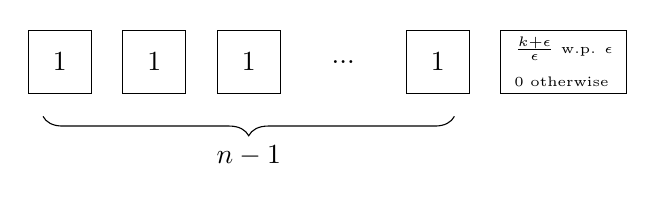
\begin{tikzpicture}[scale=0.4]
	\draw (0,0) rectangle node (C) {$1$} ++(2,2); 
	\draw (3,0) rectangle node (D) {$1$} ++(2,2); 
	%\draw (6,0) rectangle node (E) {$1$} ++(2,2); 
	\draw (6,0) rectangle node (F) {$1$} ++(2,2); 
	\draw [draw=white](9,0) rectangle node (dots) {...} ++(2,2); 
	\draw (12,0) rectangle node (A) {$1$} ++(2,2); 
	\draw (15,0) rectangle node (B)[align=left] {\tiny$\frac{k+\epsilon}{\epsilon}$ w.p. $\epsilon$\\\tiny$0$ otherwise} ++(4,2); 
	\draw[decorate,decoration={brace, amplitude=7pt, raise=13pt, mirror}]
	(C.south west) to node[black,below= 20pt] {$n-1$} (A.south east);%
	\end{tikzpicture}
	\caption{An example where the expected reward is no more than $\frac{1}{k+\ell}\sum_{j=1}^{\ell} \E [y_j]+\epsilon$}
	\label{fig:random}
\end{figure}



\section{Ranked Tie-Breaking}
\label{sec:prophet_lex}
In this section we consider the ranked tie-breaking rule, 
and present a series of single threshold strategies with their guarantees. 
We then show an interesting connection to the setting of a single agent that can choose up to $k$ rewards. 
We start by presenting the single threshold strategies.
 
\begin{theorem}\label{thm:prophet_serial_threshold_inequality}
	For every $i\leq n$ and $\ell=0, \ldots, n-i$, let $\hat{T}_i^\ell=\frac{1}{\ell+2}\sum_{j=i}^{i+\ell} \E [y_j]$. 
	The single threshold strategy $\hat{T}_i^\ell$ (i.e., select $v_t$ iff $v_t\geq \hat{T}_i^\ell$) guarantees an expected utility of at least $\hat{T}_i^\ell$ for the $i$-ranked agent.	
%For agent $i$, the threshold strategy $\hat{T}_i^\ell=\frac{1}{\ell+2}\sum_{j=i}^{i+\ell} \E [y_j]$ for $0 \leq \ell\leq n-i$  gives a $\hat{T}_i^\ell$-guarantee. 
\end{theorem}
\begin{proof}
	Fix an agent $i$. Let $S_{-i}$ be the strategies of all agents except agent $i$, and let $S=(\hat{T}_i^\ell,S_{-i})$.
	Let $\assignn{i}{j}{S}$ denote the event that agent $i$ is assigned the reward $v_j$ in strategy profile $S$. I.e., $\assignn{i}{j}{S}$ is the event that agent $i$ competed over reward $v_j$ and received it according to the ranked tie-breaking rule. 
	For simplicity of presentation, we omit $S$ and write $\assign{i}{j}$.
	We bound the utility of agent $i$ under strategy profile $S$.
	\begin{eqnarray*}
	  u_i(S)  & = & \E\left[ \sum_{j=1}^{n}{v_j\cdot\Pr\left(\assign{i}{j}\right)}\right]    \nonumber \\ 
	 & =& \E\left[\sum_{j=1}^{n}{(\hat{T}_i^\ell+v_j-\hat{T}_i^\ell)\Pr\left(v_j\geq \hat{T}_i^\ell,\forall_{r<j} \overline{\assign{i}{r}},\assign{i}{j}\right)}\right]. \nonumber 
	\end{eqnarray*}

Let $p=\sum_{j=1}^{n} \Pr(v_j\geq \hat{T}_i^\ell,\forall_{r<j}  \overline{\assign{i}{r}},\assign{i}{j})$ (i.e., $p$ is the probability that agent $i$ receives some reward in strategy profile $S=(\hat{T}_i^\ell,S_{-i})$), and let $Z^{+}=\max\{Z,0\}$.
We can now write $u_i(S)$ as follows:
\begin{eqnarray}
	 u_i(S)	  & = & p \cdot\hat{T}_i^\ell + \E\left[\sum_{j=1}^{n}{(v_j-\hat{T}_i^\ell)^+\Pr\left(\forall_{r<j} \overline{\assign{i}{r}},\assign{i}{j}\right)}\right] \nonumber \\
	& \geq & p \cdot  \hat{T}_i^\ell \label{eq:1} + \E\Bigl[\sum_{j=1}^{n}(v_j-\hat{T}_i^\ell)^+ \Bigr.  
	 \left. \cdot (1-p)\cdot\Pr\left(\assign{i}{j} \mid \forall_{r<j}\overline{\assign{i}{r}}\right)\right] \nonumber\\
%\end{eqnarray}
%\begin{eqnarray}
	& \geq & p\cdot \hat{T}_i^\ell + (1-p)\cdot \E\left[\sum_{j=i}^{n}(y_j-\hat{T}_i^\ell)^+\right] \label{eq:2}\\
	& \geq & p\cdot \hat{T}_i^\ell + (1-p)\cdot \E\left[\sum_{j=i}^{i+\ell}(y_j-\hat{T}_i^\ell)\right] \nonumber\\
	& = & p\cdot \hat{T}_i^\ell + (1-p)\cdot \left( \E\left[\sum_{j=i}^{i+\ell}y_j\right]-(\ell+1)\hat{T}_i^\ell \right)\nonumber\\
	& = & p\cdot \hat{T}_i^\ell + (1-p)\cdot \left((\ell+2)\cdot \hat{T}_i^\ell-(\ell+1)\cdot\hat{T}_i^\ell \right) = \hat{T}_i^\ell. \nonumber
	%& = & p\cdot \E\left[\sum_{j=i}^{i+\ell} \frac{y_j}{\ell+2}\right] + (1-p)\cdot\E\left[\sum_{j=i}^{i+\ell} \frac{y_j}{\ell+2}\right] = \hat{T}_i^\ell,
	\end{eqnarray}
	
	%The first inequality holds since the probability of not getting any reward until time $j$ is bounded by $1-p$ (i.e., the probability of not getting any reward). 
	%The last inequality holds since if $v_j-T^\ell\geq 0$ and agent $i$ is still active, the reward is selected, thus assigned with probability at least $1/k$. 
	
	Inequality \eqref{eq:1} holds since the probability of not getting any reward until time $j$ is bounded by $1-p$ (i.e., the probability of not getting any reward). 
	Inequality \eqref{eq:2} holds since there are at most $i-1$ agents that are ranked higher than agent $i$, therefore there are at most $i-1$ rewards that can be selected but not assigned to agent $i$.
	Finally, the last equality holds by the definition of $\hat{T}_i^\ell$.		
\end{proof}

The special case of Theorem~\ref{thm:prophet_serial_threshold_inequality} where $\ell=0$ gives the following corollary.
\begin{corollary}
For every $i$, the threshold strategy $\hat{T}_i^0$ guarantees an expected utility of $\frac{\E[y_i]}{2}$ for the $i$-ranked agent.
\end{corollary}

We next show that the bound in Theorem~\ref{thm:prophet_serial_threshold_inequality} is tight.
\begin{proposition}\label{pro:lb_serial}
	For every $\epsilon>0$ and every $i \leq n$, there exists an instance such that in the unique equilibrium of the game, the $i$-ranked agent gets an expected utility of at most $\frac{1}{\ell+2}\sum_{j=i}^{i+\ell} \E [y_j]+\epsilon$ for every $\ell \leq n-i$.
\end{proposition}

\begin{proof}
	Given some $\epsilon>0$ and $i \leq n$, consider the following instance (depicted in Figure~\ref{fig:ranked}): 
	$$
	v_t = 
	\begin{cases}
	\infty & \text{ for } t < i\\
	1 & \text{ for } i \leq t < n \\
	\frac{1+\epsilon}{\epsilon} \mbox{ w.p. } \epsilon, \mbox{ and } 0  \mbox{ w.p. } 1-\epsilon& \text{ for } t = n
	\end{cases}
	$$
	One can easily verify that in the unique equilibrium of the game, agents $1, \ldots, i-1$ will be assigned rewards $v_1,\ldots,v_{i-1}$, and agent $i$ will be assigned the last reward $v_n$ for an expected utility of $1+\epsilon$.
	It holds that:
	$$ u_i(S) = 1+\epsilon = \frac{\E[\sum_{j=i}^{i+\ell}y_j]}{2+\ell}+\epsilon.$$
\end{proof}

\begin{figure}[h!]
	\centering
	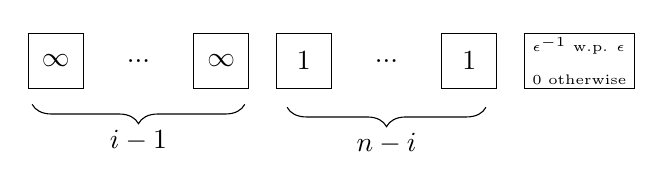
\begin{tikzpicture}[scale=0.35]
	\draw (0,0) rectangle node (G) {$\infty$} ++(2,2); 
	\draw [draw=white](3,0) rectangle node (dots) {...} ++(2,2); 
	\draw (6,0) rectangle node (J) {$\infty$} ++(2,2); 
	\draw (9,0) rectangle node (C) {$1$} ++(2,2); 
	\draw [draw=white](12,0) rectangle node (dots) {...} ++(2,2); 
	\draw (15,0) rectangle node (A) {$1$} ++(2,2); 
	\draw (18,0) rectangle node (B)[align=left] {\tiny${\epsilon}^{-1}$ w.p. $\epsilon$\\\tiny$0$ otherwise} ++(4,2); 
	\draw[decorate,decoration={brace, amplitude=7pt, raise=10pt, mirror}]
	(C.south west) to node[black,below= 16pt] {$n-i$} (A.south east);%
	\draw[decorate,decoration={brace, amplitude=7pt, raise=10pt, mirror}]
	(G.south west) to node[black,below= 16pt] {$i-1$} (J.south east);%
	\end{tikzpicture}
	\caption{An example where the expected reward for agent $i$ is no more than $\frac{1}{\ell+2}\sum_{j=i}^{i+\ell} \E [y_j]+\epsilon$}
	\label{fig:ranked}
\end{figure}

%\TBD{check if the say it or refer to it (\citet{KleinbergW19} HajiaghayiKS07 kennedy1987prophet?)}
We next show that for any instance, the set of rewards assigned to the $k$ competing agents in equilibrium coincides with the set of rewards that are chosen by the optimal algorithm for a single decision maker who can choose up to $k$ rewards and wishes to maximize their sum. 
\citet{KleinbergW19} show that the only optimal strategy of such a decision maker, takes the form of $nk$ dynamic thresholds, $\{T_t^i\}_{i,t}$ for all $t\leq n$ and $i \leq k$, so that the agent accepts reward $v_t$ if $v_t \geq T_t^i$, where $k-i$ is the number of rewards already chosen (i.e., $i$ is the number of rewards left to choose)\footnote{The uniqueness holds for distributions with no mass points. For distributions with mass points, whenever $v_t=T_t^i$, the decision maker is indifferent between selecting and passing.}. Moreover, they show that these thresholds are monotone with respect to $i$.

%Recall that this is the only optimal strategy up to cases where $v_t=T_t^i$.
%\begin{observation}[\citet{KleinbergW19}]
%	For every $t \leq n$ and $i \leq k$, $T_t^i\geq T_t^{i+1}$.
%\end{observation}

With the characterization of the strategy of a single decision maker who can choose up to $k$ rewards, we can characterize the unique SPE for the $k$-agent game\footnote{The SPE is unique up to cases where $T_j^i=v_t$; in these cases the agent is indifferent.}.
\begin{theorem}\label{thm:propht many lex is like a single agent}
Let $\{T_t^i\}_{i \in [k],t \in [n]}$ be the optimal strategy of a single decision maker who may choose up to $k$ rewards and wishes to maximize their sum. The unique SPE of the $k$-agent game is for agent $i$ to accept $v_t$ iff $v_t \geq T_t^{i'+1}$, where $i'\leq i$ is the rank of agent $i$ among the active agents. This SPE is unique up to cases where $v_t = T_t^{i'}$.
\end{theorem}
\begin{proof}
	Let $S^i$ denote the optimal strategy of the single agent who may choose up to $i$ rewards, as described above. 
	Let $S_i$ be the strategy of agent $i$ as described in the assertion of the theorem.
	We prove by induction that for every $i \in [k]$, the rewards that are chosen by agents $1,\ldots,i$ correspond to the rewards chosen by a single decision maker, who may choose up to $i$ rewards, and uses strategy $S^i$. 
	For the case of $i=1$, the claim holds trivially. %, since the settings are the same.
	Assume the claim holds for any number of agents smaller than $i$. 
	Since agent $i$ has no influence on the rewards received by agents $1,\ldots,i-1$, we may assume that agents $1,\ldots,i-1$ are playing according to strategies $S_1,\ldots,S_{i-1}$.
	
	%Let $S^i$ be the optimal strategy for a single decision maker who may choose up to $i$ awards.
	For every $i\in [k]$, the total utility of agents $1,\ldots,i$ is bounded by the utility of the single decision maker $u(S^i)$, since the single decision maker can simulate a game with $i$ competing agents. Hence, by the induction hypothesis, agent $i$ can obtain a utility of at most $u(S^i)-u(S^{i-1})$. By playing according to $S_i$, we are guaranteed that whenever at least $j$ agents are still active, any reward $v_t$ such that $v_t \geq T_t^{j}$ will be taken by one of the agents. Thus, when every agent $i$ is playing according to $S_i$, players $1, \ldots, i$ play according to $S^i$. Consequently, their total utility is $u(S^i)$, and the utility of agent $i$ is then maximal. The uniqueness (up to the cases where $v_j = T_j^{i'}$) is by the uniqueness of the optimal strategy of the single decision maker.     
\end{proof}

We note that by Theorem~\ref{thm:prophet_serial_threshold_inequality} it holds that
in the unique SPE described in Theorem~\ref{thm:propht many lex is like a single agent}, every agent  $i$ receives at least $\max_{\ell=0}^{n-i} \frac{1}{\ell+2}\sum_{j=i}^{i+\ell} \E [y_j]$. 

Using the results of \citet{alaei2011bayesian} regarding a single decision maker choosing $k$ rewards, we deduce an approximation of the social welfare in equilibrium:
%By the algorithm of \citet{alaei2014bayesian} we can deduce an approximation of the social welfare:
\begin{corollary} \label{cor:welfare_prophet}
	In SPE of the $k$ agent prophet game, the expected social welfare is at least $1-O(\frac{1}{\sqrt{k}})$ of the optimal welfare.
\end{corollary}


\section{Discussion and Future Directions}
\label{sec:future}
In this work, we study the effect of competition in prophet settings.
%
We show that under both random and ranked tie-breaking rules, agents have simple strategies that grant them high guarantees, ones that are tight even with respect to equilibrium profiles under some distributions.

Under the ranked tie-breaking rule, we show an interesting correspondence between the equilibrium strategies of the $k$ competing agents and the optimal strategy of a single decision maker that can select up to $k$ rewards. 
It would be interesting to study whether this phenomenon applies more generally, and what are the conditions under which it holds.
 



Below we list some future directions that we find particularly natural. 
\begin{itemize}
	\item Study competition in additional problems related to optimal stopping theory, such as Pandora's box \cite{weitzman1979optimal}.% and game of Googol \cite{gnedin1994solution} settings.
	\item Study competition in prophet (and secretary) settings under additional tie-breaking rules, such as random tie breaking with non-uniform distribution, and tie-breaking rules that allow to split rewards among agents.
	\item Study competition in  scenarios where agents can choose multiple rewards, under some feasibility constraints (such as matroid or downward-closed feasibility constraints). 
	\item Consider prophet settings with the objective of outperforming the other agents, as in \cite{immorlica2011dueling}, or different agents' objectives.
	\item Consider competition settings with non-immediate decision making, as in \cite{ezra2020competitive}.
\end{itemize}


\section*{Acknowledgement}
The work was partially supported by the European Research Council (ERC) under the European Union's Horizon 2020 research and innovation program (grant agreement No. 866132, 740282), and by the Israel Science Foundation (grant number 317/17).
%
% ---- Bibliography ----
%
% BibTeX users should specify bibliography style 'splncs04'.
% References will then be sorted and formatted in the correct style.
%
 \bibliographystyle{plainnat}
 \bibliography{prophet}
%
\end{document}
